% !TeX encoding = UTF-8
% !TeX root = ../main.tex

\section{结果分析与总结}

\begin{frame}{纯净语音识别结果对比}
  \small
  \begin{columns}[T]
    \column{0.56\textwidth}
    \centering
    \textbf{纯净语音识别结果}
    \vspace{4pt}

    \begin{tabular}{lcc}
      \toprule
      \textbf{方法} & \textbf{维度} & \textbf{准确率} \\
      \midrule
      MFCC-stat + KNN   & 26 维 & 80.0\% \\
      MFCC+$\Delta$/$\Delta^2$+GMM & 39 维 & \alert{100.0\%} \\
      TinyKeywordCNN (102k) & 39 维 & 95.0\% \\
      \bottomrule
    \end{tabular}

    \vspace{8pt}
    \raggedright
    \begin{itemize}
      \setlength{\itemsep}{2pt}
      \item GMM：20 条验证样本全部识别正确
      \item CNN：1 个误判（$2\to6$）
      \item KNN：4 个混淆，说明统计特征丢失了部分时序信息
    \end{itemize}

    \column{0.38\textwidth}
    \textbf{对比结论}
    \begin{itemize}
      \setlength{\itemsep}{4pt}
      \item 动态特征能补充语音变化趋势
      \item GMM 保留变长序列信息，适合小样本任务
      \item CNN 具有端到端建模能力，但本实验验证集较小
    \end{itemize}
  \end{columns}
\end{frame}

\begin{frame}{噪声鲁棒性：KNN 基线}
  \small
  \begin{columns}[T]
    \column{0.62\textwidth}
    \centering
    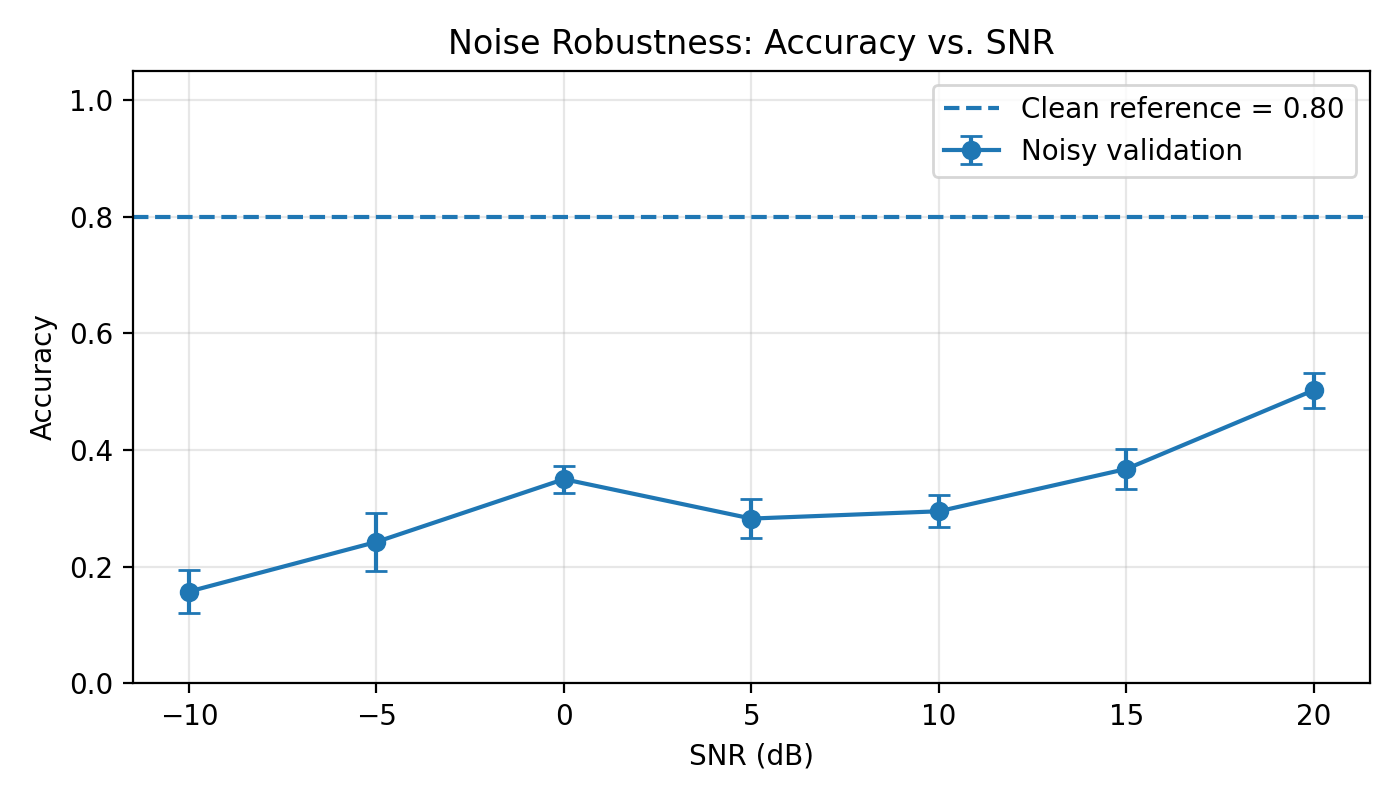
\includegraphics[width=0.95\textwidth]{../results/traditional/noise_robustness_v2/accuracy_snr_curve_mean_std.png}

    \column{0.34\textwidth}
    \textbf{MFCC-stat + KNN}
    \begin{itemize}
      \setlength{\itemsep}{4pt}
      \item 每个 SNR 重复 20 次，曲线展示均值与波动范围
      \item 低 SNR 下准确率明显下降
      \item 最高 SNR 下仍未达到 90\%，说明均值/标准差统计特征鲁棒性有限
    \end{itemize}
  \end{columns}
\end{frame}

\begin{frame}{噪声鲁棒性：GMM 序列模型}
  \small
  \begin{columns}[T]
    \column{0.62\textwidth}
    \centering
    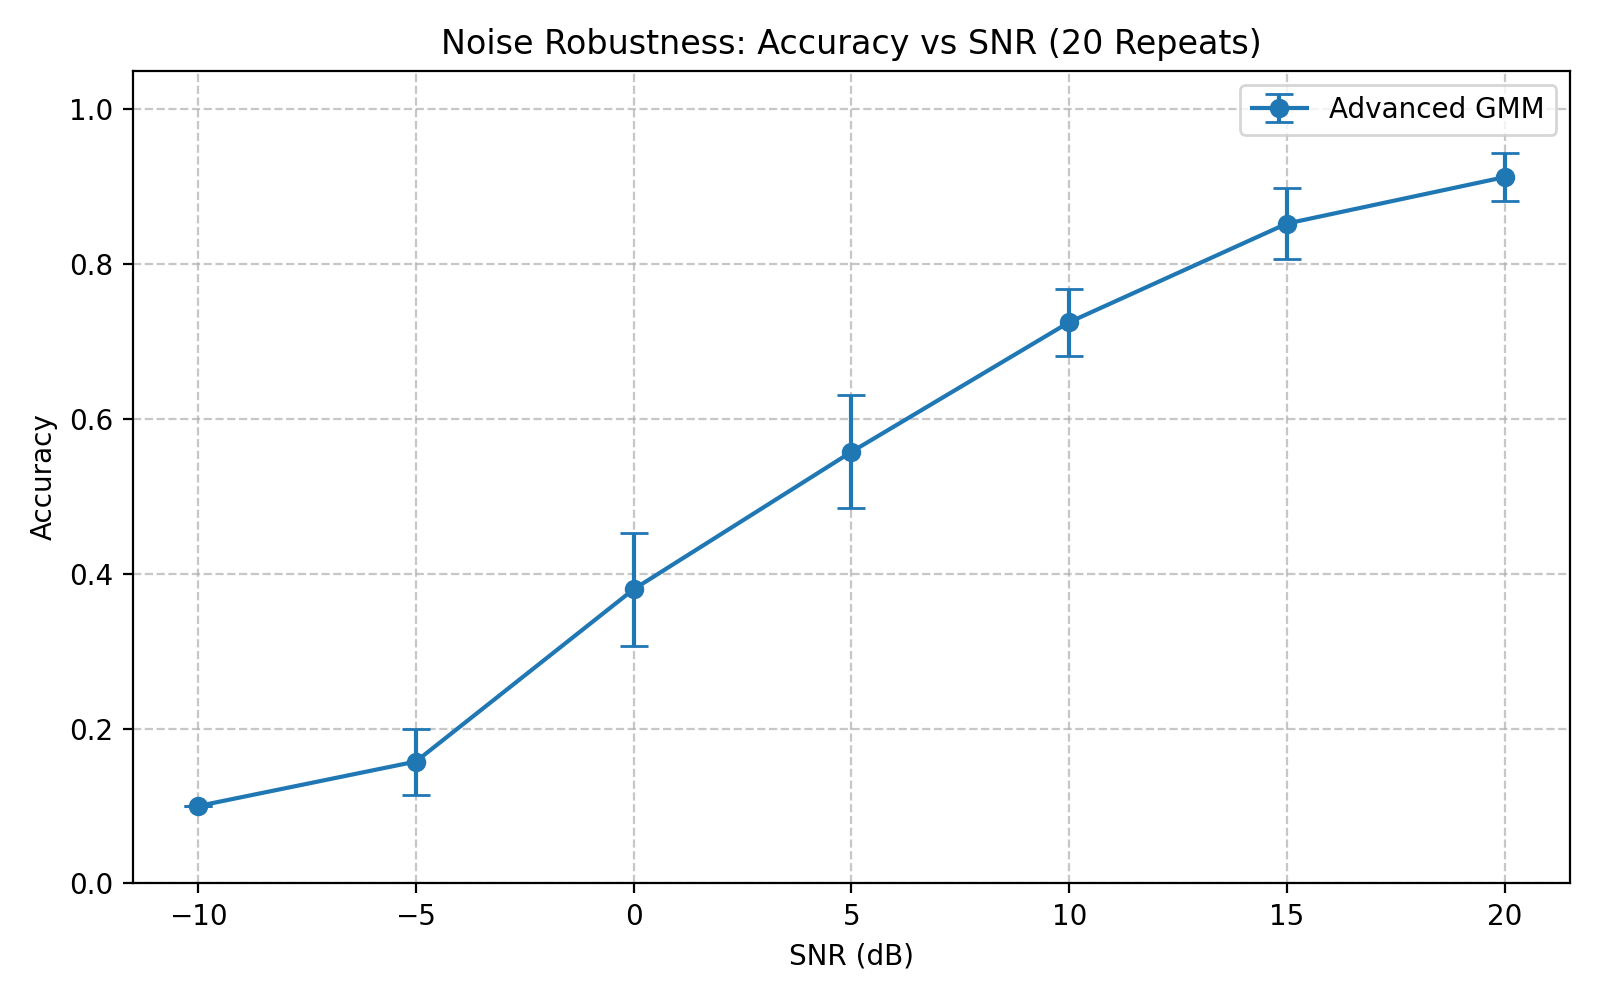
\includegraphics[width=0.95\textwidth]{../results/traditional/advanced_gmm/figures/accuracy_snr_curve.png}

    \column{0.34\textwidth}
    \textbf{MFCC + $\Delta$ + $\Delta^2$ + GMM}
    \begin{itemize}
      \setlength{\itemsep}{4pt}
      \item 引入动态特征与 CMVN 归一化
      \item 中高 SNR 下性能提升明显
      \item 在 20 dB 时达到 90\% 以上准确率（91.25\%）
    \end{itemize}
  \end{columns}
\end{frame}

\begin{frame}{噪声鲁棒性：TinyKeywordCNN}
  \small
  \begin{columns}[T]
    \column{0.62\textwidth}
    \centering
    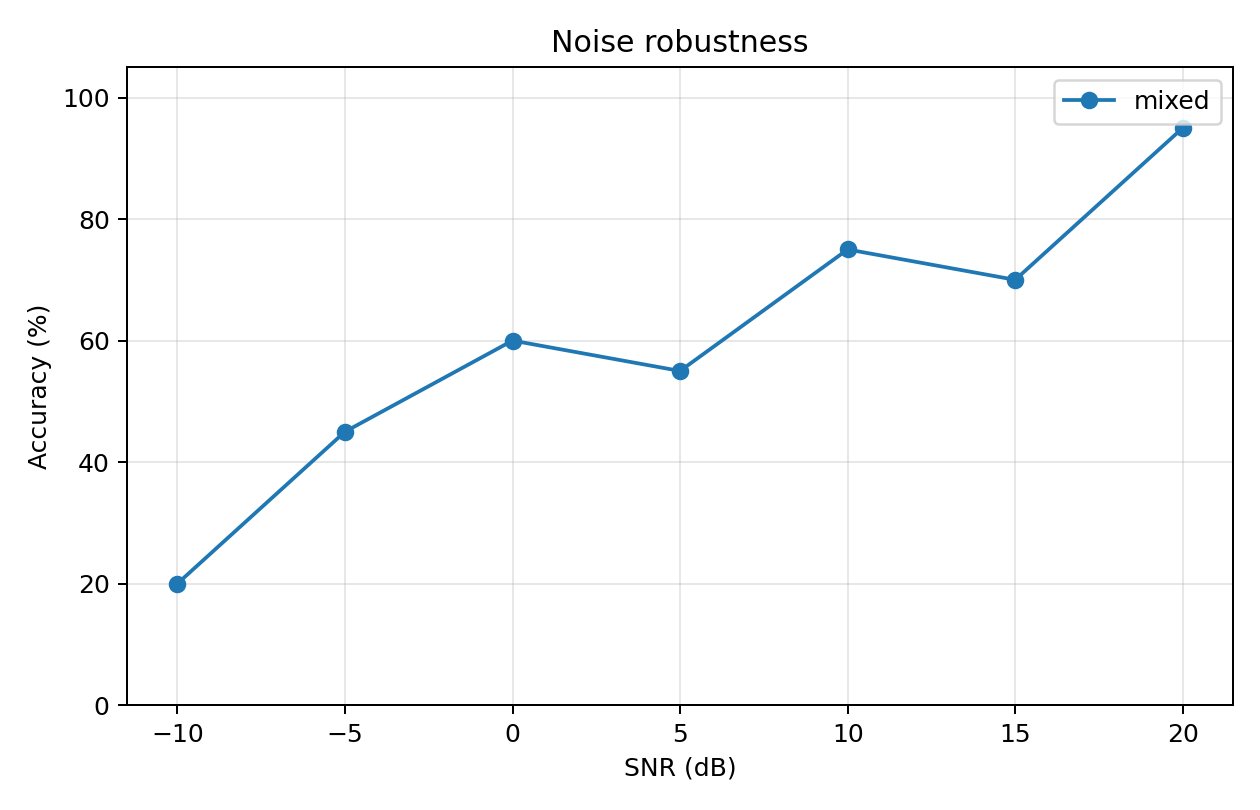
\includegraphics[width=0.95\textwidth]{../outputs/deep_learning/accuracy_snr_curve.png}

    \column{0.34\textwidth}
    \textbf{MFCC 特征图 + CNN}
    \begin{itemize}
      \setlength{\itemsep}{4pt}
      \item 训练中加入增益、平移和随机噪声增强
      \item 低 SNR 下相对更稳
      \item CNN 为单次测试，统计意义与 KNN/GMM 的重复均值不完全等价
    \end{itemize}
  \end{columns}
\end{frame}

\begin{frame}{总结与局限性}
  \footnotesize
  \begin{columns}[T,totalwidth=\textwidth]
    \column{0.51\textwidth}
    \textbf{\large 核心结论}
    \vspace{2pt}
    \begin{enumerate}
      \setlength{\itemsep}{3pt}
      \item MFCC 能有效刻画孤立数字语音的谱包络差异，是本任务的关键声学特征。
      \item KNN 基线简单可解释，但均值/标准差统计会丢失时序信息，鲁棒性较弱。
      \item GMM 保留变长序列特征，在纯净语音和中高 SNR 下表现最稳定；在 20 dB 时准确率达到 90% 以上。
      \item TinyKeywordCNN 受益于数据增强，在低 SNR 下表现相对平稳。
    \end{enumerate}

    \vspace{5pt}
    \textbf{\large 局限性}
    \vspace{2pt}
    \begin{itemize}
      \setlength{\itemsep}{2pt}
      \item 验证集仅 20 条，结果存在一定偶然性，统计意义有限
      \item 仅测试统一混合噪声，未拆分单类噪声影响
      \item 未进行说话人交叉验证
    \end{itemize}
  \end{columns}

  \textbf{\large 团队分工}
    \vspace{2pt}
    \begin{itemize}
      \setlength{\itemsep}{2pt}
      \item 于沛龙：传统方法基线、噪声鲁棒性测试、PPT 整理
      \item 景序：GMM 序列模型、传统方法优化与结果分析
      \item 封宇凡：深度学习模型设计、训练与评估
      \item 孟德轩：数据处理、实验对照、报告与展示材料整理
    \end{itemize}
\end{frame}